%
% Computer Vision - WS2013
% Abgabeprotokoll Exercise 2
%
%

%{{{ misc
\documentclass[subfigure,epsfig,fleqn,float,numbers=noenddot]{scrartcl}

\usepackage{graphicx}
\usepackage{epstopdf}
\usepackage{caption}
\usepackage{subcaption}
\usepackage{amsmath}
\usepackage[T1]{fontenc}
\usepackage[utf8]{inputenc}
\usepackage{amssymb}

\usepackage{pgfplots}

%Zitieren:
\usepackage[english]{babel}
%\usepackage[german]{babel}
\usepackage{babelbib} % f�r das Erstellen des Bibtex-Literaturverzeichnisses
\usepackage{cite}
%\selectbiblanguage{english}
%\selectbiblanguage{german}

%Peseudocode
\usepackage{algpseudocode}
\usepackage{algorithm}

%For Sourcecode
\usepackage{listings}

%Fancy shit
\usepackage{url}

\usepackage[pdftitle={Computer Vision - 2nd Exercise Round},
 						pdfauthor={Matthias Gusenbauer},
						pdfauthor={Robin Melán},
						pdfauthor={David Pfahler},
            pdfsubject={Computer Vision},
            pdfborder={0 0 0}]{hyperref}


\usetikzlibrary{plotmarks}
\pgfplotsset{compat=newest} 
\pgfplotsset{plot coordinates/math parser=false}

%%%%%%%%%%%%%%%%%%%%%%%%%%%%%%%%
% Titlepage

\pagestyle{empty}


%set dimensions of columns, gap between columns, and paragraph indent

\setlength{\textheight}{24.7 cm}
\setlength{\columnsep}{1 cm}
\setlength{\textwidth}{16 cm}
%\setlength{\footheight}{0.0 cm}
\setlength{\topmargin}{0.0 cm}
\setlength{\headheight}{0.0 cm}
\setlength{\headsep}{-0.3 cm}
\setlength{\oddsidemargin}{0.0 cm}
\setlength{\parindent}{0 cm}
\setlength{\parskip}{0.5em}
\setlength{\mathindent}{0mm}

% set page counter if document is part of proceedings
\setcounter{page}{1}
\renewcommand{\floatpagefraction}{0.9}
\renewcommand{\textfraction}{0.1}

% Set the Counters like in the exercise sheet
\setcounter{section}{3}
\renewcommand{\thesection}{Assignment \arabic{section}:}
\renewcommand{\thesubsection}{\Alph{subsection}.}

%\renewcommand{\captionlabelfont}{\fontfamily{phv}\fontseries{bx}\fontsize{10}{10pt}\selectfont}
%\renewcommand{\captionfont}{\fontfamily{phv}\fontsize{10}{12pt}\selectfont}
%\setlength{\captionmargin}{0.5 cm}

\makeatletter
\makeatother
\def\RR{\hbox{I\kern-.2em\hbox{R}}}

\begin{document}

%don't want date printed
\date{\today}

%make title bold and 14 pt font (Latex default is non-bold, 16pt) 
\title{~\\
	\fontsize{12}{12pt} \bf Computer Vision 183.585 VU 3.0 4.5 ECTS
  ~\\[0.7cm]
  \fontsize{14}{14pt} \bf 2nd Exercise Round}
  

%for single author 
\author{~\\
  ~\\
  \fontsize{12}{12pt}
  {\bf David Pfahler, Matthias Gusenbauer, Robin Melán}\\
  1126287, 1125577, 1029201
  ~\\ ~\\ ~\\
  \normalsize
}

\maketitle
%I don't know why I have to reset thispagestyle, but otherwise get page numbers 
\normalfont
\thispagestyle{empty}

%%%%%%%%%%%%%%%%%%%%%%%%%%%%%%%%%%%%%%%%%%%%%%%%%%%%%%%%%%%%%%%%%%%%%%%%%%%%%%%%
% CONTENT

\section{Image Stitching}
\label{sec:1}

\subsection{SIFT Interest Point Detection}
\label{sec:A}
As the first part of the assignment we need to extract SIFT features out of every image separately.\footnote{See Matlab-file \emph{GetSIFTFeatures.m} } Therefore we convert the image to \emph{rgb2gray(image)} and method $[text{key, desc}] = vl\_sift(siftIm);$ to extract the features from our image. The \emph{key} value consists of a 4 x n matrix, where n is the number of features found in the image, holding the x-coord., y-coord., the scale (s) factor and the orientation (in radiant). The $desc$ value holds an 128 dimensional vector for every $key$, which describe the eigenvectors (See Example in Figure \ref{img:sift}). 
	\begin{figure}[H]
		\centering
		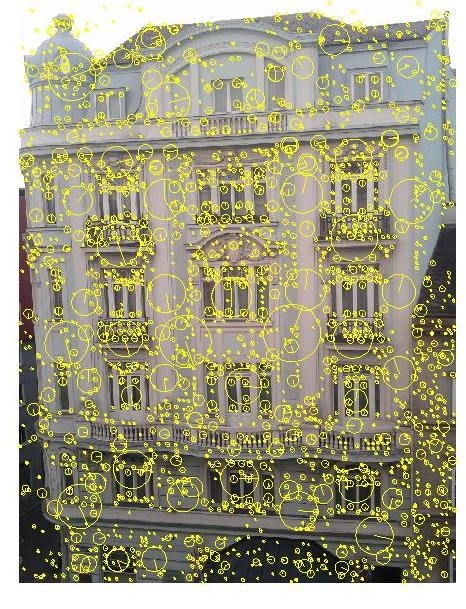
\includegraphics[width=0.55\textwidth]{./img/siftDesc2.jpg}
		\caption{Extracted Sift Features}
		\label{img:sift}
	\end{figure}

\subsection{Interest Point Matching and Image Registration}
\label{sec:B}
The next step consists of determining the homographies between all image pairs from left to right. So we start of with computing the first homography $H_\text{1,2}$ and continue until homography $H_\text{5,4}$ (I switch 5 and 4 because I need to transform the 5th image into the 4th, if I am taking the image in the middle as reference, see further \ref{sec:C}).\footnote{See Matlab-file \emph{IntPointMatching.m} } \\
To compute the homography we first need to follow a couple of steps, starting by matching our descriptors $[matches, scores] = vl\_ubcmatch(descriptor1, descriptor2);$. $Matches$ contains the indices of the original (first) and closest descriptor in the other (second) image. The $scores$ value holds the euclidean distance between them.\\
	\begin{figure}[H]
		\centering
		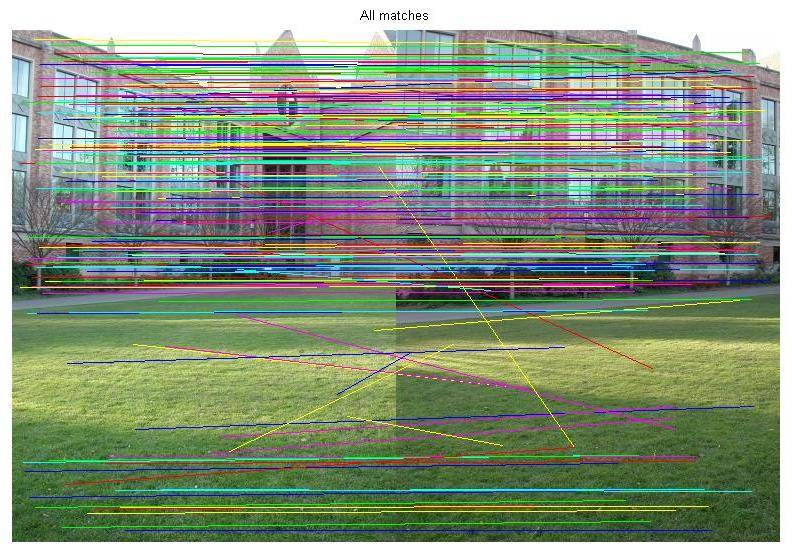
\includegraphics[width=0.85\textwidth]{./img/allMatches.jpg}
		\caption{All the Matches that where found between the two Images, as we can see some of them are outliers - therefore we need the RANSAC scheme to get rid of them, so we don't get a distorted homography at the end.}
		\label{img:outliers}
	\end{figure}
As we can see in Figure \ref{img:outliers} not all of our found matches are essentially correct, some of them are considered to be $outliers$ and if we would compute a homography including them we would get a distorted result. Therefore we apply the RANSAC scheme to receive a better estimation of the homography between the image pair.\footnote{See Matlab-file \emph{PerfRANSAC.m} } 
\par We begin by selecting randomly 4 matched-points pairwise (see Figure \ref{img:points} ) and estimate the homography between them by using the given function $cp2tform()$ as follows.
\begin{lstlisting}
$[homography] = cp2tform(rndPnts1, rndPnts2, 'projective')$. 
\end{lstlisting}
After acquiring the homography we transform all found points of interest and measure how many points are below a given threshold distance $T$ using the euclidean distance as distance metric. This is done in the function tformAInliers() in starting at line 55 in the code below. If the number of inliers in the current iteration of the algorithm is greater than the previous best result then the best homography gets updated to the current one. After $N$ iterations the inliers of the best matching homography are used to reestimate the homography which is then used to transform the image in step $C)$. 

\begin{lstlisting}[language=Matlab, numbers=left, numberstyle=\tiny]
function [ homography ] = PerfRANSAC( points1, points2 ,image1, image2, doPlot)

N = 1000;
bestInliersCnt = 0;
bestInliers = 0; 
bestHomo = 0;


for(i=1:N)
    randoms = randsample(size(points1, 1),4);
    
    rndPnts1 = points1(randoms,:);
    rndPnts2 = points2(randoms,:);
        
    try
        % b) - d)
        [nrInliers, inliers, TFORM] = tformAInliers(points1, points2, rndPnts1, rndPnts2);
        
        % if new calculation is better than old update result
        if(nrInliers > bestInliersCnt)
            disp(sprintf('Best match - #of inliers \%d', nrInliers));
            bestInliersCnt = nrInliers;
            bestInliers = inliers; 
            bestHomo = TFORM;
        end
        
    catch err
        disp('Ouch!');
    end
end

% 4) after N runs take best homography and reestimate with all points
% saving only the inliners from points1 and 2
m1 = zeros(bestInliersCnt,2);
m2 = zeros(bestInliersCnt,2);

pos = 1;
for i = 1:size(bestInliers,1)
    if (bestInliers(i) == 1)
        m1(pos,:) = points1(i,:);
        m2(pos,:) = points2(i,:);
        pos = pos + 1;
    end
end

% Output all inliers:
if (doPlot)
    match_plot(im2double(image1{1,1}), im2double(image2{1,1}), m1, m2);
    title('Matches of only Inliers!');
end
[~, ~, homography] = tformAInliers(points1, points2, m1, m2);

end

function [ nrInliers, inliers, homography ] = tformAInliers( points1, points2, rndPnts1, rndPnts2)

T = 5;

% b) estimate transformation ob rndPnts1 onto rndPnts2
homography = cp2tform(rndPnts1, rndPnts2, 'projective');

% c) transform the points 
trnsfrmdPnts = tformfwd(homography, points1(:,1), points1(:,2));

% d) calc euclidean distance
distance = (trnsfrmdPnts - points2).^2; %one line sqrt(sum(.))
distance = sqrt(distance(:, 1) + distance(:, 2));

% Thresholding
inliers = distance<=T;
nrInliers = sum(inliers);

end
\end{lstlisting}

	\begin{figure}[H]
		\centering
		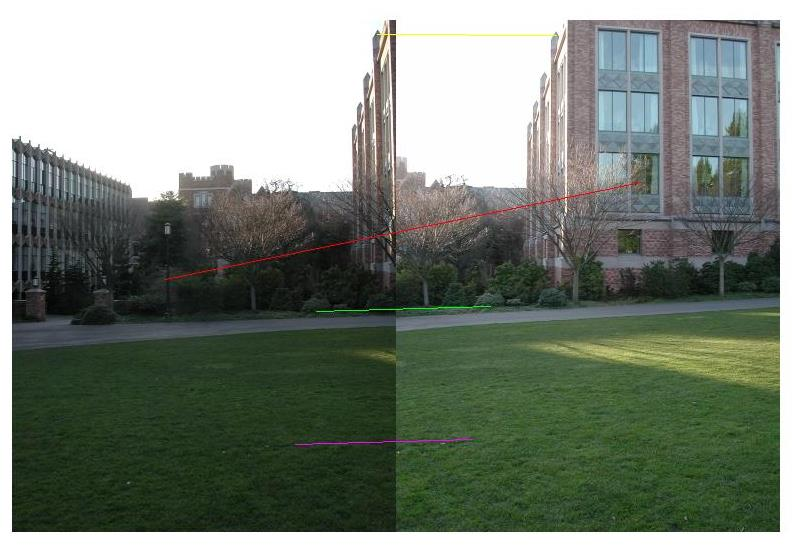
\includegraphics[width=0.55\textwidth]{./img/fourRandomMatches.jpg}
		\caption{Select randomly 4 matched-points}
		\label{img:points}
	\end{figure}

\subsection{Image Stitching}
\label{sec:C}
So after we determined the homographies between all the image pairs we select the image in the middle (in our case Image 3) to be our reference image and compute all homographies that map the other images to our reference:
\begin{equation*}
\\H_{1,3} = H_{2,3} * H_{1,2} \\
H_{5,3} = H_{4,3} * H_{5,4} 
\end{equation*}
Before we can stitch our images into one panorama picture we need to compute the size the output image is going to have. For this information we can take the method $imtransform$ with our new homographies and as a result we get the new size (xData, yData) of the transformed image, which is saved in our case for all 4 images (we don't need to compute the reference image, because we know it is going to be in the middle of the panorama picture) in an array: 
\begin{lstlisting}
	%% saves the dimensions of all the transformed images
	xLim = zeros(4,2);
	yLim = zeros(4,2);
	
	[transImage, xLim(1,:), yLim(1,:)] = imtransform(Images{1}, H_1_3);
	...
	
	%% Getting the Coordinates for final Image
	xMin = min(min(xLim));
	xMax = max(max(xLim));
    
	yMin = min(min(yLim));
	yMax = max(max(yLim));
    
	%% Width and Height of panorama image.
	width  = round(xMax - xMin);	
	height = round(yMax - yMin);
\end{lstlisting}

Now that we know the output dimensions of our final panorama image we can transform all of our images into that particular size by using again the $imtransform$ method but this time adding our appropriate dimensions [xMin xMax] and [yMin yMax] as our XData and YData parameters. Given all transformed images, the final step is to blend them together in a way to avoid seams. To do this we use an $\alpha$ channel where the value of $\alpha$ for an image is 0 at all border pixels and 1 at the maximum distance from the border. The remaining values are linearly interpolated (see Figure \ref{img:bwdist}). For Example our interpolation value $\alpha$ would look like Figure \ref{img:interpolation}. the final color at a pixel in the output image is computed as the $\alpha$-weighted sum of overlapping images. More precisely, if there are $n$ images overlapping at pixel position $(x,y), I_i(x,y), i = 1...n$ with color $(R_i,G_i,B_i)$ and weighting factors $\alpha_i$, the color values in the stitched output image O are computed as:
\begin{equation*}
	O(x,y) = \frac{\sideset{}{_{i=1}^n}\sum_{} (R_i,G_i,B_i) * \alpha_i} {\sideset{}{_{i=1}^n}\sum_{} \alpha_i}
\end{equation*}
This blending method is called $feathering$.
	\begin{figure}[H]
		\centering
		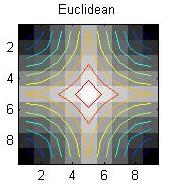
\includegraphics[width=0.75\textwidth]{./img/bwdist.jpg}
		\caption{To compute our $\alpha$ channel we used the method $bwdist$ with the euclidean distance method}
		\label{img:bwdist}
	\end{figure}
	\begin{figure}[H]
		\centering
		
\includegraphics[width=0.75\textwidth]{./img/interpolationFactor.jpg}
		\caption{$\alpha$ channel for panorama picture}
		\label{img:interpolation}
	\end{figure}
	
\paragraph{Results}
Our first set of images $campus1...5.jpg$ with $feathering$:
\begin{figure}[H]
		\centering
		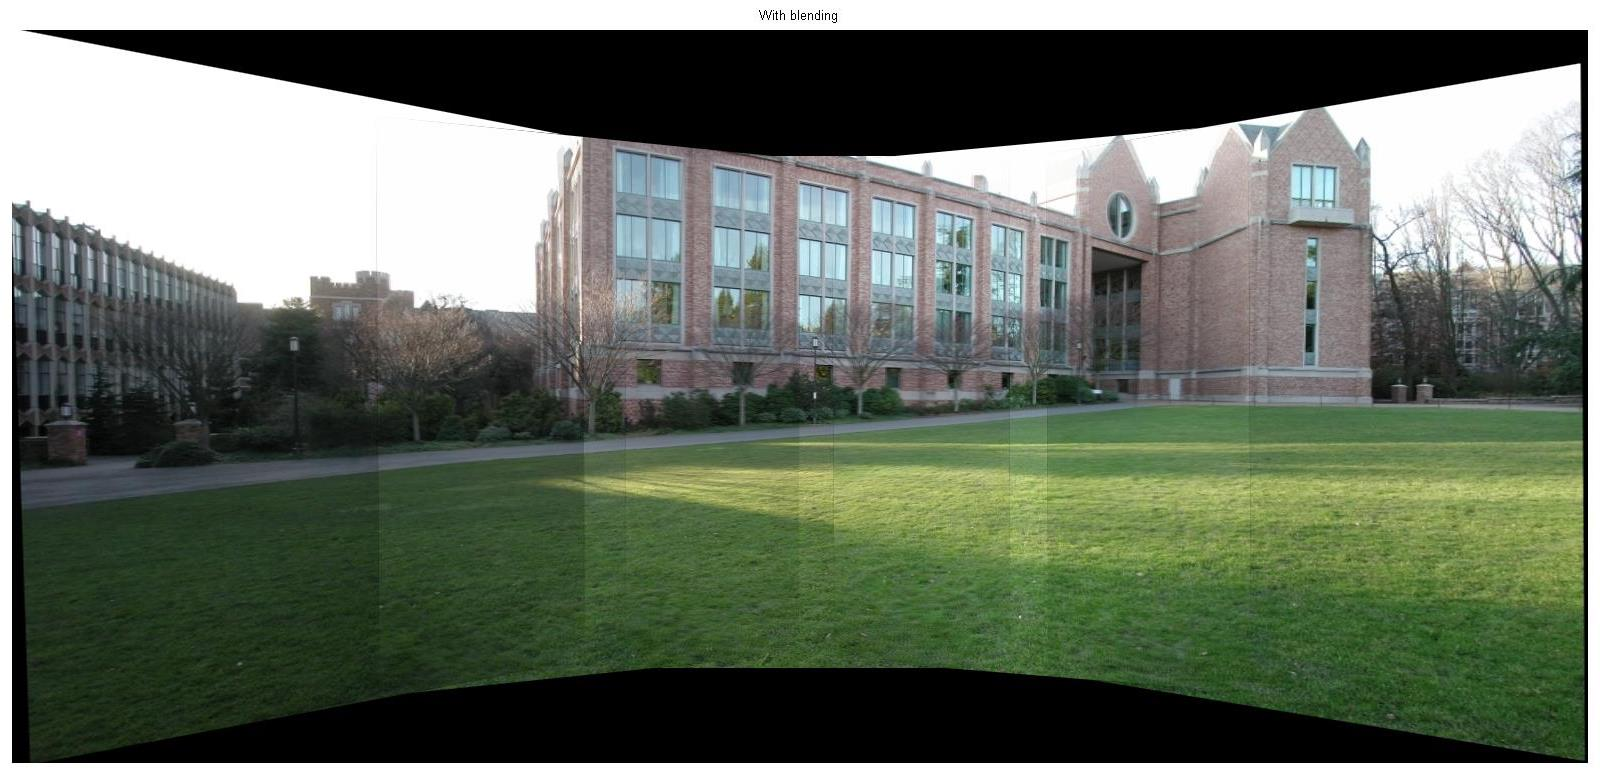
\includegraphics[width=0.95\textwidth]{./img/withBlending.jpg}
		\caption{}
		\label{img:withBlend}
\end{figure}
And without $feathering$ (the transformed images are laid over each other from left to right):
\begin{figure}[H]
		\centering
		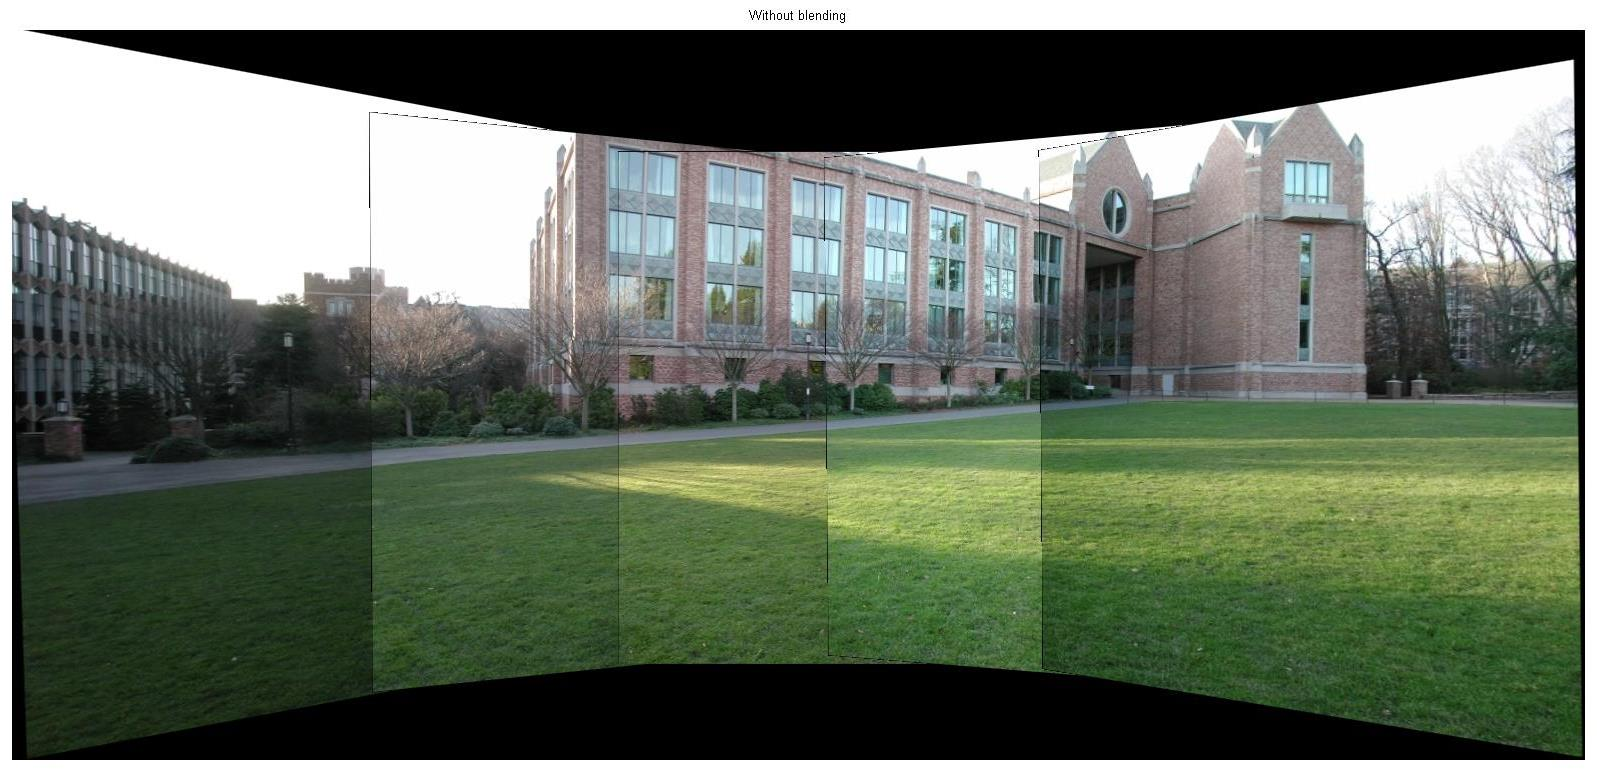
\includegraphics[width=0.95\textwidth]{./img/withoutBlending.jpg}
		\caption{}
		\label{img:withoutBlend}
\end{figure} 
Our second set of images $officeview1...5.jpg$ with $feathering$:
\begin{figure}[H]
		\centering
		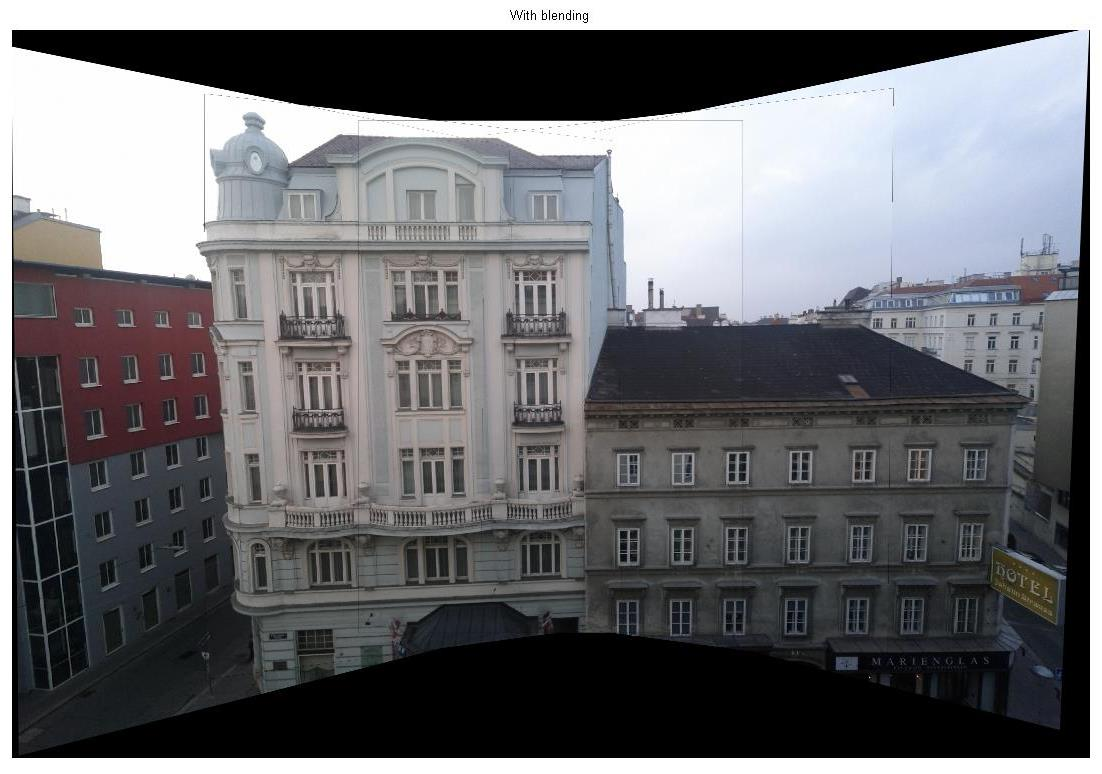
\includegraphics[width=0.95\textwidth]{./img/withBlending2.jpg}
		\caption{}
		\label{img:withBlend2}
\end{figure}
And without $feathering$ (the transformed images are laid over each other from left to right):
\begin{figure}[H]
		\centering
		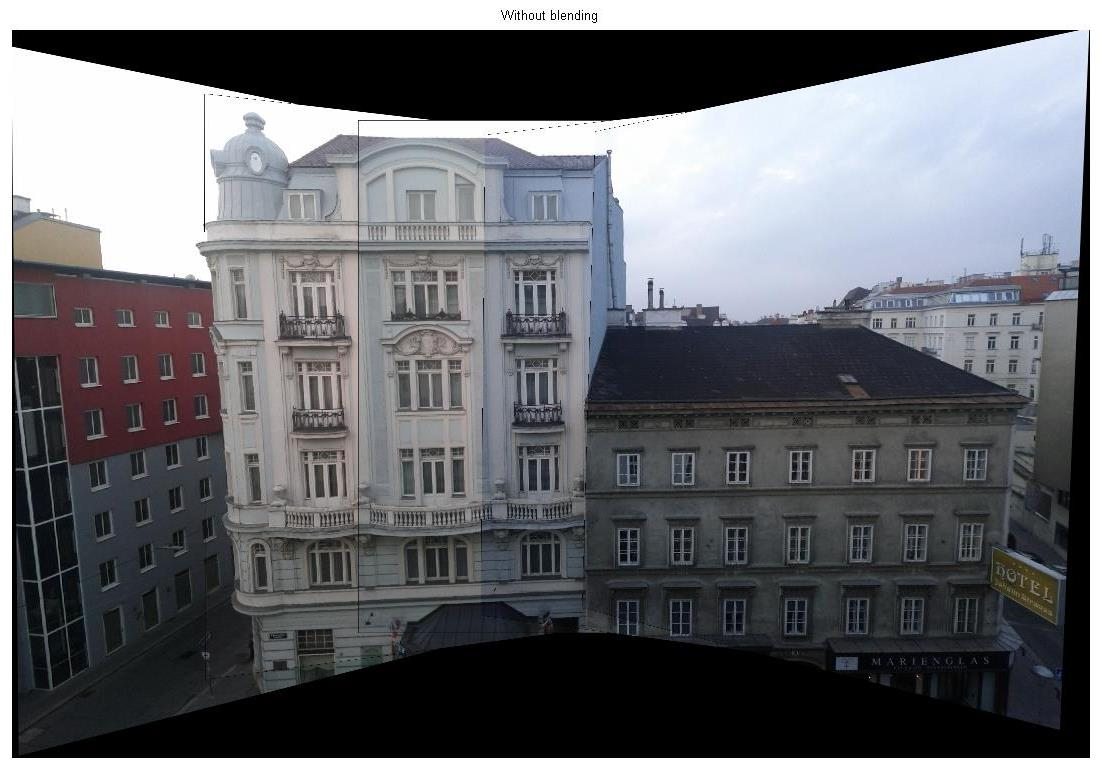
\includegraphics[width=0.95\textwidth]{./img/withoutBlending2.jpg}
		\caption{}
		\label{img:withoutBlend2}
\end{figure}

Especially looking at the first image we see that some of the images could not be overlaid correctly, which means that there still were some small outliers which distorted the homography so that the final image is at some parts a little blurry. 
With the second sample we detect the $feathering$ effect much better than for the first image because the shading through the image is continuous. 

\pagebreak
\section{Scene Recognition with Bag of VisualWords}
\label{sec:2}

\begin{figure}
		\centering
		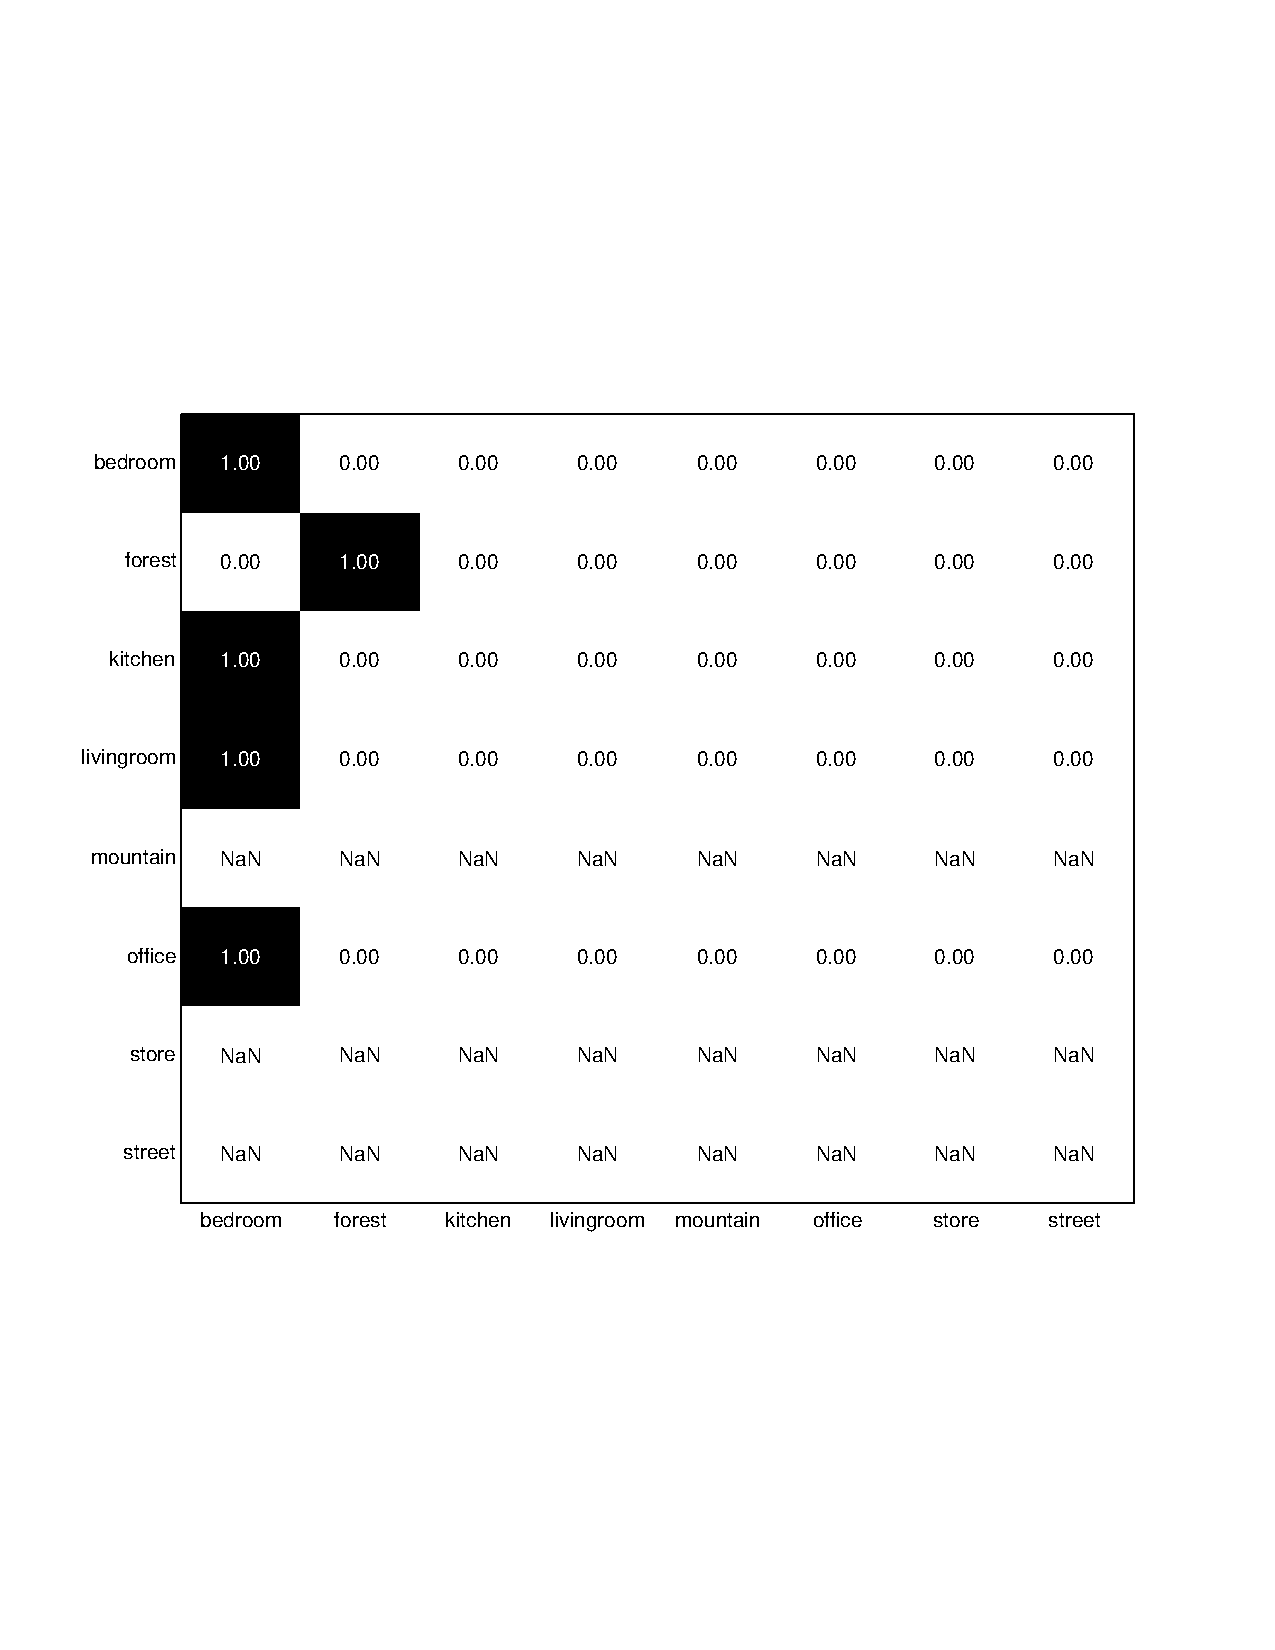
\includegraphics[width=\textwidth]{img/conf_matrix_own.pdf}
		\caption{Conf Matrix Own}
		\label{fig:conf_matrix_own}
\end{figure}
\begin{figure}
		\centering
		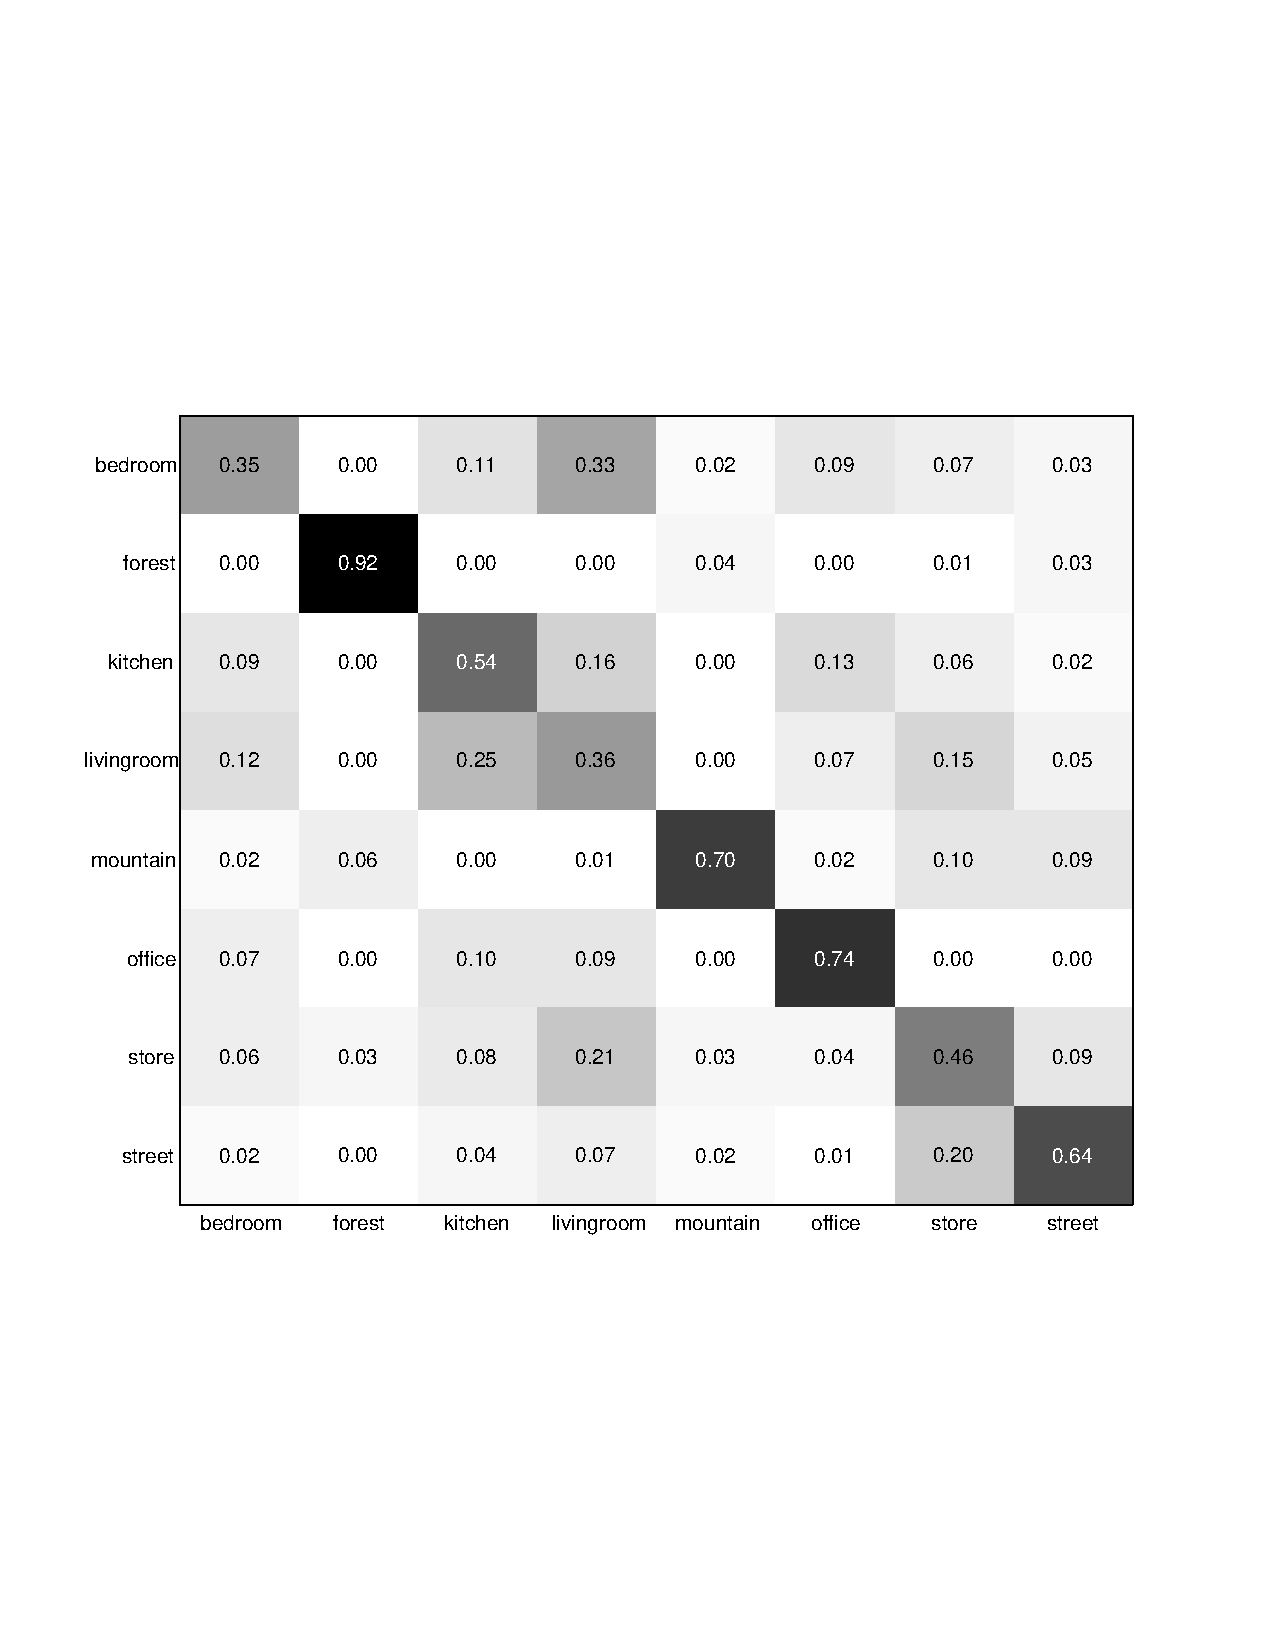
\includegraphics[width=\textwidth]{img/conf_matrix_test.pdf}
		\caption{Conf Matrix Test}
		\label{fig:conf_matrix_test}
\end{figure}

\end{document}

% vim:foldmethod=marker
